\documentclass[12pt]{report}
\usepackage{float}
\usepackage{emptypage}
\usepackage{graphicx}
\usepackage{float}
\usepackage[section]{placeins}
\usepackage[a4paper, margin=1in, left=1.4in]{geometry}
\usepackage{rotating}
\usepackage{verbatim}
\usepackage{listings}
\usepackage{ragged2e}
\usepackage{array}
\usepackage{tocbibind}
\usepackage[colorlinks=true,linkcolor=black]{hyperref}
\usepackage[export]{adjustbox}
\usepackage{rotfloat}
\usepackage{fancyhdr}
\usepackage{etoolbox}
\usepackage{multicol}

\usepackage{tikz}
\usetikzlibrary{calc}
\usetikzlibrary{decorations.pathmorphing}

\graphicspath{ {./img/} }

\usepackage[toc,acronym]{glossaries}
\makeglossaries

\newacronym{urc}{URC}{University Rover Challenge}
\newacronym{gps}{GPS}{Global Positioning System}
\newacronym{ssh}{SSH}{Secure SHell}
\newacronym{rgb}{RGB}{Red-Green-Blue}
% \newacronym{RGB-D}{Red-Green-Blue-Depth}
\newacronym{tcp}{TCP}{Transmission Control Protocol}
\newacronym{udp}{UDP}{User Datagram Protocol}
\newacronym{lan}{LAN}{Local Area Network}
\newacronym{gui}{GUI}{Graphical User Interface}
\newacronym{ir}{IR}{InfraRed}
\newacronym{lidar}{LIDAR}{LIght Detection And Ranging}



\begin{document}
\pagenumbering{gobble}

\title{Major Project Report}
\author{AS Karthik, Abhishek Krishna, Gagan Deep G}


\begin{tikzpicture}[overlay,remember picture]
    \draw [line width=1mm,decorate,decoration={lineto}]
        ($ (current page.north west) + (0.9in,-0.5in) $)
        rectangle
        ($ (current page.south east) + (-0.5in,0.5in) $);
\end{tikzpicture}

\begin{center}
	\textbf {
		\Large R.V. COLLEGE OF ENGINEERING\\
		\Large BENGALURU - 560059\\
		\small(Autonomous Institution Affiliated to VTU, Belagavi)\\[1cm]
	}
	
\includegraphics[scale=0.25]{rvcelogo.png}\\[1cm]
	\Large \textbf{CCTV Video Summarisation in Urban Environments}\\[1cm]
	\large \textbf{PROJECT REPORT} \\[0.5cm]
	\normalsize Submitted by\\

	\begin{multicols}{2}
		\begin{flushright}
			\large \textbf{AS Karthik}\\
			\large \textbf{Abhishek Krishna}\\
			\large \textbf{Gagan Deep G}
		\end{flushright}

		\columnbreak

		\begin{flushleft}
			\large \textbf{1RV15CS001}\\
			\large \textbf{1RV15CS007}\\
			\large \textbf{1RV15CS053}
		\end{flushleft}
	\end{multicols}

	\bigskip

	\normalsize \textbf{Under the Guidance of}\\

	\begin{multicols}{2}

		\normalsize \textbf{Dr. Ramakanth Kumar P}\\
		\normalsize Professor \& HoD\\
		\normalsize Dept. of CSE, RVCE\\
		\normalsize Bengaluru - 560059\\

		\columnbreak

		\normalsize \textbf{External Guide Name}\\
		\normalsize Designation\\
		\normalsize Company Name\\
		\normalsize Bengaluru - 5600XX\\

	\end{multicols}

	\bigskip
	\medskip

	\normalsize \textbf {In the partial fulfillment for the award of degree of}\\
	\normalsize \textbf {\textit{Bachelor of Engineering}}\\ in \\
	\normalsize \textbf {COMPUTER SCIENCE \& ENGINEERING \\ 2018-19}

\end{center}



\newpage


\begin{tikzpicture}[overlay,remember picture]
    \draw [line width=1mm,decorate,decoration={lineto}]
        ($ (current page.north west) + (0.9in,-0.5in) $)
        rectangle
        ($ (current page.south east) + (-0.5in,0.5in) $);
\end{tikzpicture}

\begin{center}
	\textbf {
		\Large R.V. COLLEGE OF ENGINEERING\\
		\Large BENGALURU - 560059\\
		\small(Autonomous Institution Affiliated to VTU, Belagavi)\\[0.3cm]
	}
	
\includegraphics[scale=0.2]{rvcelogo.png}\\[0.3cm]
		\Large \textbf{\underline {CERTIFICATE}}\\
\end{center}
\linespread{1.2}\normalsize \begin{center} \justify
Certified that the major project work titled \textbf{<Project Name>} has been carried out by \textbf{AS Karthik (1RV15CS001), Abhishek Krishna (1RV15CS007) \& Gagan Deep G (1RV15CS053)} who are bonafide students of R.V. College of Engineering, Bengaluru in partial fulfillment for the award of degree of Bachelor of Engineering in Computer Science and Engineering of the Visvesvaraya Technological University, Belagavi during the year 2018 - 2019. It is certified that all corrections/suggestions indicated for the internal assessment have been incorporated in the report deposited in the departmental library. The major project report has been approved as it satisfies the academic requirements in respect of project work prescribed by the institution for the said degree.
\end{center}

\linespread{1}

\begin{center}

	\medskip
	\begin{multicols}{3}

		\columnbreak

		\hrulefill\\
		\small \textbf{Dr. Ramakanth Kumar P}
		\small{
			\\ Professor,
			\\Department of CSE,
			\\RVCE, Bengaluru - 59
		}\\

		\columnbreak

		\hrulefill\\
		\smallskip
		\small \textbf{Dr. Ramakanth Kumar P}
		\small{
			\\Prof. \& Head of Department,
			\\Department of CSE
			\\RVCE, Bengaluru - 59
		}\\

		\columnbreak

		\hrulefill\\
		\smallskip
		\small  \textbf{Dr. Subramanya KN}
		\small{
			\\Prinicpal,
			\\RVCE, Bengaluru - 59
		}\\
	\end{multicols}


	\bigskip
	\bigskip
	\large \textbf{External Viva}
	\begin{multicols}{2}

		\begingroup
			\leftskip2em
			\rightskip2em

			\normalsize \textbf{Name of the Examiners}
			\\
			\bigskip
			1. \hrulefill\\
			\bigskip
			2. \hrulefill\\

		\endgroup

		\columnbreak

		\begingroup
			\leftskip2em
			\rightskip2em

			\normalsize \textbf{Signature with Date} \\
			\bigskip
			1. \hrulefill\\
			\bigskip
			2. \hrulefill\\
		\endgroup


	\end{multicols}
\end{center}


\newpage


\begin{tikzpicture}[overlay,remember picture]
    \draw [line width=1mm,decorate,decoration={lineto}]
        ($ (current page.north west) + (0.9in,-0.5in) $)
        rectangle
        ($ (current page.south east) + (-0.5in,0.5in) $);
\end{tikzpicture}

\begin{center}
	\textbf {
		\large R.V. COLLEGE OF ENGINEERING \\
		\large BENGALURU - 560059\\
		\small(Autonomous Institution Affiliated to VTU, Belagavi)\\[1cm]
	}
	\Large \textbf{\underline {DECLARATION}}\\[1cm]
\end{center}
\linespread{1.5}\normalsize \begin{center} \justify
We, \textbf{AS Karthik (1RV15CS001), Abhishek Krishna (1RV15CS007) \& Gagan Deep G (1RV15CS053)}, students of Eighth Semester B.E., Computer Science and
Engineering, R.V. College of Engineering, Bengaluru hereby declare that the major
project titled \textbf{Project Name} has been carried out by us and submitted in partial
fulfillment for the award of degree of Bachelor of Engineering in Computer Science
and Engineering of Visvesvaraya Technological University, Belagavi during the
academic year 2018-2019. We declare that matter embodied in this report has not been submitted to any other university or institution for the award of any other degree or diploma.
\end{center}
\linespread{1}

\begin{multicols}{2}

	\begin{center}
		\begingroup
			\leftskip2em
			\rightskip2em

			\normalsize \textbf{Place : Bengaluru} \\
			\medskip
			\textbf{Date: }\hrulefill\\
		\endgroup
	\end{center}

	\columnbreak

	\begin{center}
		\begingroup
			\leftskip2em
			\rightskip2em

			\textbf{Signature}\\
			\bigskip
			1. \hrulefill\\
			\bigskip
			2. \hrulefill\\
			\bigskip
			3. \hrulefill\\
		\endgroup
	\end{center}


\end{multicols}

\cleardoublepage

\pagenumbering{roman}


\addcontentsline{toc}{chapter}{Acknowledgement}

\begin{center}
	\huge\bfseries Acknowledgement
\end{center}

\bigskip

Any achievement, be it scholastic or otherwise does not depend solely on the individual efforts
but on the guidance, encouragement and cooperation of intellectuals, elders and friends.
A number of personalities, in their own capacities have helped us in carrying out this project work.
We would like to take this opportunity to thank them all. \bigskip

We deeply express my sincere gratitude to our guide Dr. Ramakanth Kumar P, Professor,
Department of CSE, R.V.C.E, Bengaluru, for his able guidance, regular source of encouragement and assistance
throughout this project. \bigskip

We would like to thank Dr. Ramakanth Kumar. P, Prof. \& Head of Department,
Computer Science \& Engineering, R.V.C.E, Bengaluru, for his valuable suggestions and expert advice.\bigskip

We also extend our cordial thanks to Company name, for providing us an opportunity to carry out the internship in its organization. We also would like to thank my external guide Name, manager and all team members for their support and guidance.\bigskip

We would like to thank Dr. Subramanya. K. N, Principal, R.V.C.E, Bengaluru, for his moral support towards completing our project work.\bigskip

We thank our Parents, and all the Faculty members of Department of
Computer Science \& Engineering for their constant support and encouragement.\bigskip

Last, but not the least, we would like to thank my peers and friends who
provided us with valuable suggestions to improve our project.

\pagebreak

\addcontentsline{toc}{chapter}{Abstract}
\begin{center}
	\huge\bfseries Abstract

	\bigskip
	\normalsize

	\justify
	The use of CCTVs has been on the steady rise in in the last decade, being used for the security of public and private establishments alike. With increasing crime rates in cities, there is a need for a smarter method to survey the video being recorded, rather than manually going through hours of footage, saving both time and labour. We propose to an efficient method to generate a summary of the footage. The project also aims to simplify the task further, by generating video summaries based on user query, thus showing exactly what is required. \\

	The process has been carried out in two phases, real-time and query phase. Real-time phase works on the raw CCTV footage working to detect motion, separate the foreground and background, extract this "tube of interest and store it. YOLO object detector is then run on the these tubes and the metadata is also stored. The query phase works on this intermediate data. The user selects the objects (ex: car, bike etc)  required in the summary. The required events are then selected, before being rearranged by an optimization algorithm like Simulated Annealing. A background of the input footage is simultaneously generated along with these processes. Finally, the rearranged tubes are blended into the background using poisson blending to generate the summary video. \\

	Both objective and subjective parameters have been used to evaluate the results. Objectively, the exhaustiveness (inclusion of all events), compression factor, and overlap factor have been considered. A compression factor of 4-5x was successfully achieved, while all significant events were selected to achieve excellent exhaustiveness. All trials also successfully managed to attain very less overlap factor, of less than 0.1. Subjectively, semantic structuring and realisticity of the footage were considered. Interacting events were always shown together(thereby maintaining semantic structuring). The blending of the tubes could however be better leading to a more realistic video.

\end{center}

\bigskip



\pagebreak

\cleardoublepage

\tableofcontents
\listoffigures
\listoftables
% \printglossary[type=\acronymtype,style=long,title=Glossary,nonumberlist]

\cleardoublepage

% \printnoidxglossary[type=\acronymtype,title=Glossary]



\pagenumbering{arabic}

\pagestyle{fancy}
\fancyhf{}
\fancyhead[LEO]{Chapter \thechapter}
\fancyhead[REO]{CCTV Video Summarisation}
\fancyfoot[L]{Dept. of CSE, RVCE}
\fancyfoot[C]{2018 - 2019}
\fancyfoot[R]{\thepage}
\renewcommand{\headrulewidth}{1.25pt}
\renewcommand{\footrulewidth}{1.25pt}

\patchcmd{\chapter}{\thispagestyle{plain}}{\thispagestyle{fancy}}{}{}


\chapter{Introduction}

Introduction

\section{State of the art developments}

\section{Purpose}

\section{Objective}

\section{Scope}

\section{Motivation}

\section{Organization of Report}

\section{Summary}

\chapter{Overview of Video Summarization}

After having gone through several important papers in this sector, we have narrowed down to follow the framework described in this section. It mainly has two phases: Real-Time Phase and Query Phase.


\section{Real-time phase}
The real-time phase reads the cctv footage, identifies clips of interest and performs certain image processing algorithms on the footage of interest to extract “flow-tubes” and tags from clips and stores them in a database. The phase is split into the following steps:

\begin{enumerate}
    \item \textbf{Motion Detection}

    Detect motion in the footage and identify any clips with significant motion while disregarding artefacts due to changing environmental conditions and other insignificant disturbances.
    MOG is used in this step to see if there is any movement, and if there is significant foreground present in an image, decided by a static threshold, we consider the clip to have motion in it. MOG is specifically useful here due to its dynamic nature and adaptability to gradual changes in the environment very quickly and, additionally, availability of efficient parallel CUDA implementations of this very effective algorithm.

    \item \textbf{Background Masking}

	A foreground extractor like a Mixture of Gaussians is used to extract the subjects of interests in the clips identified by motion detection.
    The same technique used in previous step is also employed here to generate foreground masks and thereby just extracting the foreground. Several techniques were experimented on and it turns MOG is the best cost effective and accurate technique available for our specific needs.

    \item \textbf{Computation of Objects flow-tubes}

	Flow-tubes are computed from the extracted foreground in previous phase.
    Flow tubes are extracted by performing morphological operations and several redundant foreground blobs are removed in this step. Furthermore, individual subjects present in each frame are identified, and related back with the subjects present in the previous frame, thereby producing flow-tube arrays.

    \item \textbf{Object Tagging}

	After actual subjects are identified in the previous phase, the subjects are classified into several popular categories using a popular deep-learning model called “You Only Look Once” model, and these tags are computed.
	We use a pre-trained 26-layered YOLOv3 model as the most common categories present in a common CCTV video footage are already present in the set of categories identifiable on a YOLOv3 trained on the standard COCO dataset.

    \item \textbf{Metadata storage}

    In this stage, a connection is established to the database and the tags and flow-tubes computed are stored into the database.
\end{enumerate}

\section{Query Phase}

The query phase processes the user input query, extracts the relevant tubes and generates a relevant summary. This phase is split into the following steps:

\begin{itemize}

    \item \textbf{Tube Selection}

    The user query containing various parameters such as time period, tags and length of summary required are taken from user and relevant flow-tubes are selected from the database.
    This stage is easily implemented by writing logic to create a query with all the parameters the user specifies in the input query.

    \item \textbf{Rearrangement}
    An optimisation algorithm, in our case simulated annealing, is used to rearrange the flow-tubes in the time dimension to produce a summary of the desired length.

    While there are several heuristic based search algorithms are recommended for these purposes by different authors, simulated annealing remains to be the most successful and most popularly cited method. Hence, we have implemented simulated annealing with a custom cost function based on our needs.

    \item \textbf{Time-lapsed background generation}
    In this step a background is generated based on the time period and summary length required by user.
    A weighted approach, with the periods where there is most activity, is considered more heavily in generating the time-lapsed background.

    \item \textbf{Blending}
    Poisson blending is used to blend the rearranged flow-tubes with the time-lapsed background to generate the summary we require. This summary is then saved onto the user’s computer.
\end{itemize}

\section{Summary}
In this chapter, we have given an overview of how our solution to the problem statement of summarizing CCTV video footage is structured. However there is no strict constraints on following the above prescribed framework for solving this problem. In our view, this structure optimizes the amount of time required to generate summaries and also help in rapid prototyping and validating of various techniques/models during the course of developing the application.
\chapter{Software Requirement Specification of CCTVVS}

Software Requirements Specification is detail description of system behavior
that is constructed. It integrates the functional and nonfunctional requirements
for software to be constructed. The functional requirements describe what
exactly the software must do and the non-functional requirement includes the
constraint on the design or implementation of the system. A function is
described as a set of inputs, the behavior, and outputs. A non-functional
requirement is a requirement that specifies criteria that can be used to judge
the operation of a system, rather than specific behaviors.

\section{Overall Description}

This section describes the general factors which affects system and the
requirements. The software developed should provide means to configure order
assignment, generate master files with required restrictions and must handle
concurrent assignment of orders to reconciliation specialists. This section
also deals with user characteristics, constraints on using the system and
dependencies of the system on other applications.

    \subsection{Product Perspective}
    The system should be versatile and easy to use. It should be flexible and
    the response time should be quick. The system is composed of several modules
    performing different tasks and they must be well co-ordinated. The system
    developed should be easy to deploy and maintain. The intended end users for
    this are mostly CCTV operators and security managers. The system must be
    self-explanatory as it will be used by laymen or people with minimum
    technical experience.

    \subsection{Product Functions}
    The sole purpose of the product is to generate semantic, concise and
    relevant summaries for the specified time periods. The product must be
    versatile enough to handle sophisticated queries which considers several
    parameters like type of subjects, time period, summary length, degree of
    importance of events, duration of events to be considered etc.

    \subsection{User Characteristics}
    The end users of the system are mostly of to two roles, CCTV operators and
    security managers. Since they are not technical specialists, the user
    interface is expected to be simple and easy to use. It can be assumed that
    the general user of this application is versed in form-based inputs and has
    a grasp on basic English to use the interface accordingly. It is also
    assumed that the user can make all kinds of queries, both valid and invalid,
    and it is up to to the software to validate the queries and provide
    responsive feedback accordingly.

    \subsection{Constraints and Dependencies}
    The dependencies and constraints that the project has are:
    \begin{itemize}
        \item The first major constraint is the memory constraint. The number
        of flow-tubes it can hold in memory is directly proportional to the
        amount of events which can be optimized at a time.
        \item The system is highly dependent on having accurately tuned
        hyper-parameters, whether it be the threshold for motion detection or
        the learning (exploration/exploitation) rate used in the optimization
        technique, must be tuned specifically for each use-case.
        \item The number of categories it can recognize in a video is
        constrained on the diverseness of the dataset used to train the
        deep learning model used.
        \item A major dependency of the project is the \gls{openCV} parallel
        implementation of several advanced algorithms like MOG and Poisson
        Blending.
    \end{itemize}

\section{Specific Requirements}

This section covers all software requirements with sufficient details to be made
use of by the designers to build a system to satisfy requirements. The product
perspective and user characteristics do not state the actual requirements needed
that the system but rather state how the product should work with respect to
user convenience. The specific requirements are actual data with which the
customer and software provider can agree. The final system is expected to
satisfy all the requirements mentioned here.

    \subsection{Functional Requirements}
    The functional requirements of the system are:
    \begin{itemize}
        \item The system must automatically validate user queries before
        processing them
        \item The system must produce video summaries based on the user query
        given
        \item The system must label each event shown in summary with relevant
        time stamps
        \item The system must be able to identify and tag events in real-time
        \item The system must be able to merge and rearrange events without
        losing meaning
        \item The system must be able to seamlessly blend subjects with
        generated time-lapsed background
        \item The system must be able to generate a relevant background based on
        the density of events distributed across the queried period of time
        \item The system must be able to generate summaries not longer than ten
        percent of the queried period length
        \item The user query form must be versatile enough to encompass all
        forms of relevant queries
        \item The system must have a feature to manually tune the various
        possible hyper-parameters from the user interface
    \end{itemize}

    \subsection{Performance Requirements}
    Performance requirements for the system include the following:
    \begin{itemize}
        \item The system should be able to transmit the video feed with minimal
        loss of packets
        \item The delay with respect to the video transmission should be minimal
        \item The control signal should be transmitted at real time
        \item The obstacle detection should happen in real time
    \end{itemize}

    \subsection{Supportability}
    The UI will be web-based and hence can be used on any system. While the
    system is built on python and open-source tools which are ubiquitous in
    modern day PCs, however it is recommended to use computers with large amount
    of RAM for fast performance, as the algorithm developed for optimization
    requires the system to hold significantly large arrays in memory.

    \subsection{Software Requirements}
    The different software requirements required by the application are as
    follows:
    \begin{itemize}
        \item Operating System:
        \begin{itemize}
            \item OS X Yosemite and higher versions
            \item Windows 7 and higher versions
            \item Linux 16.04 LTE and higher
        \end{itemize}
        \item Platform: Python Virtual Environment
        \item Language: Python
        \item Interface: Python GUI
        \item IDE/tool:
        \begin{itemize}
            \item Visual Studio Code
            \item Jupyter Notebook
        \end{itemize}
    \end{itemize}

    \subsection{Hardware Requirements}
    The various hardware requirements of the system are:

    \begin{itemize}
        \item Platform/CPU
        \begin{itemize}
            \item Modern multi-core processor (Ex: Intel Core i7 6700HQ) on
            x86/ARM platform
        \end{itemize}
        \item Memory
        \begin{itemize}
            \item Minimum: 8GB
            \item Recommended: 16GB or higher
        \end{itemize}
        \item Storage
        \begin{itemize}
            \item 64GB or higher for storing an entire day of video (depending
            on video resolution)
        \end{itemize}
    \end{itemize}

    \subsection{Design Constraints}
    The system is designed to be versatile and flexible. The design constraints
    include a user friendly interface. It should be able to handle requests in
    short time periods. The system must ensure that database is always in a
    consistent state. Also, the system must be built to handle all possible
    inputs so as to make the feature comprehensive enough for non-technical
    end users. The system must be able to validate input queries.

    \subsection{Interfaces}
    This section describes the interfaces in detail. The two types of
    interfaces involved are User Interfaces and Software Interfaces.
        \subsubsection{User Interfaces of the system}
        There is a single user interface from which the software accept
        parameters from the user and downloads the summary created. It must be
        form based and have the following parameters:
        \begin{itemize}
            \item Input source \& output file path
            \item Time period
            \item Summary length
            \item List of tags of subjects to include
            \item Learning rate
            \item Threshold for size of events
        \end{itemize}

        \subsubsection{Software Interfaces of the system}
        The following software interfaces are implemented in the application:
        \begin{itemize}
            \item The different modules developed in the system uses standard
            pre-defined data structures as interfaces between each other.
            \item Each module is developed as objects hence, the data
            internally is exposed by helper functions.
        \end{itemize}


    \subsection{Non-Functional Requirements}
    These are the requirements that specify criteria that can be used to judge
    or evaluate the operation of the system rather than specific behavior and
    are not directly concerned with the specific functions delivered by the system.

    \begin{itemize}
        \item Efficiency: The system shall perform at best possible efficiency
        in all internal operations.
        \item Availability: The system must be up and running at all times and
        must accommodate users
        \item Security: The system must be well built with no security threats.
        \item Uniformity: The system must perform on any standard browser and
        any OS in the same way, while producing fairly similar summaries each
        time a similar query is made.
        \item Speed: The system must have a short latency period and must be
        responsive
    \end{itemize}

\section{Summary}

The specific requirements and constraints that must be kept in mind while
building the application have been detailed in this chapter. These include the
hardware requirements, software requirements and functional requirements for
automation of reconciliation. Also, this chapter cites the various assumptions
being made by the developer of the system for auto assignment of orders.  All
these have to be managed while building and running the system.
\chapter{High Level Design}
Design is significant phase in development of software. It is basically a creative procedure which includes the description of the system organization, establishes that it satisfies the functional and non-functional system requirements. Larger systems divided down into smaller sub-systems contain services that are related to each other. The output in design phase describes the architecture of software to be used for the development of the common endpoint service. This section depicts the issues that are required to be covered or resolved before attempting to devise a complete design solution. The detailed design includes an explanation for all the modules. It throws light on the purpose, functionality, input and output. The software specification requirements have been studied to design an appropriate and efficient software to handle a multitude of users belonging to different user groups simultaneously accessing the system.

\section{Design Considerations}
There are several design consideration issues that need to be fixed before designing a solution for the system to be implemented. The following sections describe constraints that have heavy impact on the software, a method or approach used for the development and the architectural strategies. It also describes the overview of the system design.

    \subsection{General Constraints}
    General constraints which need to be considered are:

    \begin{itemize}
    \item The user should have access/authorization to use the system
    \item The user should have knowledge of the required inputs and the formats of the inputs
    \item The system must be tuned for the use-case before using it

    \end{itemize}

    \subsection{Development Methods}
    The design method employed is highlighted in this chapter. The data flow model has been the design method employed for development of the system. A data flow model is modeling system based on data transformation that takes place as the data is being processed. The notations used represent functional processing and data stores. Data flow models gives the better understanding of how data is associated with the particular process by tracking and providing the documentation.

    We have split up the project into independent modules which can be independently developed, tested and validated.


\section{Architectural Strategies}
The overall organization of the system and its high level structure is provided by this section and this section also provides the key insight into the mechanism and strategies used in system architecture. The overall architecture was designed keeping in mind the need for rapid-prototyping required for a project of this scale which needs to be accomplished in a fairly short period of time.

    \subsection{Programming Language}
    The system involves two major segments, the frontend and backend which are built using Python, Javascript, HTML, CSS. Python is a object oriented programming languages which support wide range of data types and application programming interface for handling the data. The user interfaces are developed using HTML, CSS and JavaScript.

    Other important packages which were vital for developing this project were OpenCV implementations of several image processing algorithms, Jupyter’s interactive python interpreter and NumPy package used for performing fast and vectorized operations on images.

    \subsection{User Interface Paradigm}
    The GUI of the system is a form based interface. It is light-weight and fairly simple to develop. However, it is built to only take valid input queries from the user. Therefore the UI paradigms which we wish to achieve are consistency, clarity and simplicity.

    \subsection{Error Detection and Recovery}
    Error detection and recovery is an important aspect of the implemented project. We have implemented user form validation in the very beginning of the pipeline. Almost all kinds of errors will be weeded out in the very beginning of the pipeline. Internal error detection is done using the exception handling clauses provided by Python and using plenty of datatype asserts wherever possible. Since the project is divided into clearly defined modules with pre-defined interfaces, debugging and detecting errors is very easy.

\section{System Architecture}
This section is focused on basic structure of model in the system. It aims to identify major modules in system and communication flow amongst these modules. The approach used for the development of the common endpoint service is object oriented wherein the system is classified into different objects, which represent real world entities. The architecture is depicted in the figure below.

\begin{figure}[H]
    \centering
    \includegraphics[scale=0.45]{uml.png}
    \caption{UML Class Diagram}
    \label{img:uml}
\end{figure}

The system architecture is as shown in Figure \ref{img:uml}. The central summarizer object creates objects other modules mentioned in the figure and uses them in a sequence mentioned in chapter 2. Each constructor of the classes defined above, have strict assert statements to ensure the data they receive are of the proper type before any kind of operations are performed on them.

\section{Data Flow Diagram}

A Data Flow Diagram (DFD) is graphical representation of the "flow" of data through an information system. Data Flow models describe how data flows through a sequence of processing steps. DFD is composed of four elements, which are process, data flow, external entity and data store. With data flow diagram, the users can easily to visualize the operations within the system, what can be accomplished using the system and implementation of the system. DFDs provide the end users an abstract idea regarding the data that is given as input to the system, the effect that the input will ultimately have upon the whole system.

The level 0 diagram shows the main data streams in the system. The level 1 diagram shows the input and output data in the two main processing pipelines. The level 2 diagram explains the data transformation in each pipeline step-by-step.

    \subsection{Data Flow Diagram – Level 0}

    The level 0 DFD describes general operation of the system. It represents the system and user and the inputs and outputs between the user and the system.

    \begin{figure}[H]
        \centering
        \includegraphics[scale=0.2]{dfd-lvl-0.png}
        \caption{Data Flow Diagram - Level 0 }
        \label{img:dfd-lvl-0}
    \end{figure}

    Figure \ref{img:dfd-lvl-0} gives an abstract representation of the system. The input video from CCTV is fed into the Summarizer which gives the video summary as output, based on the query from the CCTV operator/user.


    \subsection{Data Flow Diagram – Level 1}

    The Level 1 DFD describes the system more in detail than the Level 0 DFD. It specifies the two main phases involved in the system. This is as shown in fig \ref{img:dfd-lvl-1}.

    \begin{figure}[H]
        \centering
        \includegraphics[scale=0.2]{dfd-lvl-1.png}
        \caption{Data Flow Diagram - Level 1 }
        \label{img:dfd-lvl-1}
    \end{figure}

    The real-time phase takes in the input video from the CCTV camera and processes the data for the next phase. Different methods like motion detection, background masking, tube extraction and object detection are applied on the given input video. The pre-processed data is then stored in the database. Next, a query is given as input for the next phase. Using the preprocessed data from phase one, a summarized video is generated.

    \subsection{Data Flow Diagram – Level 2}

    Figures \ref{img:dfd-lvl-21}, \ref{img:dfd-lvl-22} represent the level 2 data flow diagrams.

    The processes in level 1 are expanded here. The Level 2 DFD for Real-time phase of the video summarizer is shown in figure \ref{img:dfd-lvl-21}.

    \begin{figure}[H]
        \centering
        \includegraphics[scale=0.2]{dfd-lvl-21.png}
        \caption {Data Flow Diagram - Level 2 (Depth image processing)}
        \label{img:dfd-lvl-21}
    \end{figure}

    Motion is first detected frame by frame be using a threshold of number of active pixels in the binary mask. From these clips of interest, the foreground is extracted using MOG2. Events of interest are then extracted as tubes. YOLO object detector is then applied to these tubes to create tagged even tubes which are stored in the database. Simultaneously, a static background is generated from the input footage, which is also stored.

    \begin{figure}[H]
        \centering
        \includegraphics[scale=0.2]{dfd-lvl-22.png}
        \caption {Data Flow Diagram - Level 2 (Colour image processing)}
        \label{img:dfd-lvl-22}
    \end{figure}

    Figure \ref{img:dfd-lvl-22} shows level 2 DFD for Query phase of the Video Summarizer. Based on the user query, tubes of interest are first selected from the database. These tubes are then rearranged using Simulated Annealing.. While this process is being completed, a time-lapsed background is also formed. In the next step, the rearranged tubes are blended into the time-lapsed background by Poisson blending. The generated summarized video is then stored.

\section{Summary}
The above data models depict how data is processed by the system. This constitutes the analysis level. The notations applied above represent functional processing, data stores and data movement amongst the functions. The purpose of chapter is to describe major high- level processes (the two phases – Real time and Query) and their interrelation in the system. All the above mentioned levels of DFDs illustrate these.
\chapter{Detailed Design}
In the Detailed Design phase, the internal logic of every module specified in High Level Design (HLD) is determined. Specifically, in this phase the design of each module, the low-level components and subcomponents are described. After determining HLD graphical representation of the software system being developed is drawn. Each module‘s input and output type, along with the possible data structures and algorithms used are documented during the detailed design phase. The following sections provide such information of the modules.

\section{Structure Chart}
The structure chart shows the control flow among the modules in the system. It explains all the identified modules and the interaction between the modules. It also explains the identified sub-modules. The structure chart explains the input for each modules and output generated by each module.

In the system, there are six sub modules. They are Video file reader, Background creator, Motion Detector, Tube generator, Tube rearrangement module and Summary maker. The description of the sub modules, the flow of data and the results of each sub module are shown in Figure \ref{img:structure-chart}. The modules each receive input and process the input and produce output which is seen to end users in a web dashboard.

The video is read from an input source, frame by frame, it is then sent to the motion detection module and identified as either clip of interest or ignored. These clips are then processed to extract useful information such as tags and flow-tubes which are then stored into a database. Further, when a query is made, relevant flow-tubes are gathered, rearranged and a relevant background is simultaneously generated. These two are then seamlessly blended to produce the summary.


\begin{figure}[H]
    \centering
    \includegraphics[scale=0.4, angle=90]{structure-chart.png}
    \caption{Structure Chart}
    \label{img:structure-chart}
\end{figure}

\section{Functional Description of Modules}
The internal working of certain core modules is explained in this section. It also describes the software component and subcomponent of the system.

    \subsection{Motion Detection Module}
    This is the main module of the system which is responsible identifying clips of interest in a sparse CCTV footage.

    \begin{itemize}
        \item \textbf{Purpose:} The purpose of this module is to decide whether each frame is relevant or not.
        \item \textbf{Input:} The input to this module are frames of input video source and timestamp .
        \item \textbf{Output:} The output is whether the input should be saved for further processing or ignored.
        \item \textbf{Functionality:} The functionality of this module is to detect motion and save those clips of interest.
        \item \textbf{Flowchart:} The flowchart shown in figure \ref{img:flowchart-motion} explains the motion detection module. The module starts by reading a frame and applies the stored MOG model onto the frame. If the generated background mask has more foreground pixels than a specified threshold then it is considered as a frame with motion and is stored as clip of interest.
    \end{itemize}

    \begin{figure}[H]
        \centering
        \includegraphics[scale=0.7]{flowchart-motion.png}
        \caption{Motion Detection Flowchart}
        \label{img:flowchart-motion}
    \end{figure}


    \subsection{Background Creation Module}
    This is the second module of the system which is responsible for the generation of a time-lapsed background.

    \begin{itemize}
        \item \textbf{Purpose:} The purpose of this module is to generate a timelapsed background for the input time-period and specified duration to overlay the rearranged flow-tubes.
        \item \textbf{Input:} The input is a stream of frames in the specified time-period, and length of summary which is required to overlay on this background.
        \item \textbf{Output:} A background clip representing the background for the given duration condensed into a clip as long as the rearranged summary generated.
        \item \textbf{Functionality:} The module implements a queue type buffer, which is continuously updated and median value for each pixel row in the buffer is calculated and stored as background.
        \item \textbf{Flowchart:} The flowchart shown in the Figure \ref{img:flowchart-background} explains the procedure followed in the Background creation module. The module uses a buffer which stores the history of  frames from previous 4 minutes or more, depending on the length of summary, and background is calculated by pixelwise calculation of the median across the whole buffer. The buffer is updated as new frames are read into the queue data structure. The median implementation is parallelized to optimize performance.
    \end{itemize}

    \begin{figure}[H]
        \centering
        \includegraphics[scale=0.7]{flowchart-background.png}
        \caption{Background Creation Flowchart}
        \label{img:flowchart-background}
    \end{figure}


    \subsection{Optimisation Module}
    This is module of the system handles the optimization and rearrangement of selected tubes.

    \begin{itemize}
        \item \textbf{Purpose:} The purpose of this module is to rearrange tubes and produce a compact meaningful summary.
        \item \textbf{Input:} 3D arrays of flow-tubes extracted and their original timestamps.
        \item \textbf{Output:} The module computes an optimal configuration of the flow-tubes based on a pre-defined cost function to generate the summary.
        \item \textbf{Functionality:} The module generates an optimized configuration of flow-tubes which is both condense yet meaningful in nature.
        \item \textbf{Flowchart:} The flowchart shown in the Figure \ref{img:flowchart-optimisation} explains the procedure followed in the optimization module. We have used a popular heuristic based search algorithm to implement this module called Simulated Annealing. The algorithm trades-off from exploration to exploitation as the number of iterations and epochs increases.  The module uses a pre-defined cost function to evaluate a fitness score for each configuration and the global optimized configuration (GOC) is updated as per the sigmoid value obtained from applying the sigmoid function on the difference in fitness value from the current and previous globally optimized configurations. Higher the sigmoid value, higher are the chances of the GOC getting updated.
    \end{itemize}


    \begin{figure}[H]
        \centering
        \includegraphics[scale=0.5]{flowchart-optimisation.png}
        \caption{Optimisation Module Flowchart}
        \label{img:flowchart-optimisation}
    \end{figure}


    \subsection{Tube Extraction Module}
    This module of the system which handles the extraction of flow-tubes of several subjects present in the clips of interest identified by motion detection module.

    \begin{itemize}
        \item \textbf{Purpose:} The purpose of this module is to identify and extract flow-tubes from each clip of interest.
        \item \textbf{Input:} 3D arrays of MOG masks of video frames of the clips of interest.
        \item \textbf{Output:} 3D arrays of masks which represent the flow-tubes for each subject tracked in each clip of interest.
        \item \textbf{Functionality:} The module identifies flow-tubes whose length is beyond the specified user-threshold and extracts the flow-tubes as mask arrays and stores them for further processing later.
        \item \textbf{Flowchart:} The flowchart shown in the Figure \ref{img:flowchart-tube} explains the procedure followed in the tube extraction module. The module’s core component is the connected component search implementation. Each frame is processed to identify the number of individual blobs present in the frame and are correlated with the blobs seen in the previous frame to track existing subjects and create new subjects as and when they occur in each clip of interest. After having individually identified each subject by annotating the subjects as such in the input video feed, individual mask flow-tube arrays are created for each subject and then stored with their respective timestamps.
    \end{itemize}

    \begin{figure}[H]
        \centering
        \includegraphics[scale=0.7]{flowchart-tube.png}
        \caption{Tube Extraction Flowchart}
        \label{img:flowchart-tube}
    \end{figure}

\section{Summary}
The internal working of the application’s three modules with the necessary data flow through each of them has been described in this chapter. A clear view on control flow within system was conveyed by the structure chart with the functionality of its modules being explained. The flow charts explain the working of each module with flow of control in the module specified which gives a complete understanding of the functioning.
\chapter{Implementation of CCTVVS}

The implementation phase is significant phases in the project development as it
affords final solution that solves the issues. In this phase the low level
designs are transformed into the language specific programs such that the
requirements given in the software requirements specification are satisfied.
This phase entails actual implementation of ideas that were described in
analysis and design phase. The technique and the methods that are used for
implementing software must support reusability, ease of maintenance and should
be well documented.

\section{Modules and Classes}
We have split the code into different functional modules for easy development,
testing and maintenance of the code.

\begin{figure}[H]
    \centering
    \includegraphics[scale=0.37]{uml.png}
    \caption{Classes / Modules of CCTVVS}
    \label{img:uml}
\end{figure}

The classes of the summarisation system are as shown in Figure \ref{img:uml}.
The central summariser object creates objects other modules mentioned in the
figure and uses them in a sequence mentioned in chapter 2. Each constructor of
the classes defined above, have strict assert statements to ensure the data they
receive are of the proper type before any kind of operations are performed on
them.

\section{Algorithms}

    \subsection{Simulated Annealing Algorithm}
    Algorithm \ref{algorithm:simulated-annealing} shows the simulated annealing algorithm
    which is used for the tube optimisation process.

    \begin{algorithm}
        \SetAlgoLined
        \KwResult{Optimised Configuration}
        Let \(Config_{current} = Config_{inital}\);
        \For {\(T \gets T_{max}\) \KwTo \(T_{min}\)}{
            \(E_{current} = E(C_{current})\)
            \(C_{next} = next(C_{current})\)
            \(E_{next} = E(C_{next})\)
            \(\Delta E = E_{next} - E_{curr}\)
            \uIf { \(\Delta E > \theta\)}{
                \(C_{current} \gets C_{next}\)
            }\uElseIf {\(e^{\frac{-\Delta E}{T}} > rand(0,1)\)}{
                \(C_{current} \gets C_{next}\)
            }
        }
        \caption{Simulated Annealing}
        \label{algorithm:simulated-annealing}
    \end{algorithm}

    \subsection{Tube Extraction Algorithm}
    Algorithm \ref{algorithm:tube-extraction} shows the tube extraction algorithm
    which is used for the extracting the event tubes from the labelled motion
    volume.

    \begin{algorithm}
        \SetKwInput{in}{input}
        \SetAlgoLined
        \KwResult{3D space-time volume with connected labelled events}
        \tcc{a 3d array representing the time-space volume with foreground
        represented as 1 and background as 0}
        \in{VideoMask}

        \(volume \gets empty\_list()\)
        \(tube\_num \gets 0\)
        \(prev\_frame \gets zeros\_like(VideoMask[1])\)
        \(prev\_count \gets 0\)

        \For {\(Frame in VideoMask\)}{
            \(labelled\_frame, count = findConnectedComponents(Frame)\)

            \For{\(i in range(0,count)\)} {
                \(matches \gets empty\_list()\)
                    \For{\(j in range(0, prev\_count)\)}{
                        \If { \(\frac{Sum((labelled\_frame[k==i]*prev\_frame))}
                        {Sum(prev\_frame)} > Threshold\) }{
                            \(matches.append(j)\)
                        }
                    }
                \(matches\_dict[i] \gets matches\)
            }

            \(prev\_frame \gets Frame\)
            \(prev\_count \gets count \)

            \For {\(region in match\_dict\)}{
                \If{\(len(match\_dict[region]) \textgreater 1\)}{

                    \For{\(index in match\_dict[region]\)}{
                        \For{\(frame in volume\)}{
                            \tcc{Update labels of tubes in previous frame}
                            \(frame[frame == index] = tube\_num\)
                        }

                        \tcc{Update the dict}
                        \(match\_dict[region] = [tube\_num]\)
                    }
                }
            }

            \tcc{There are no intersection issues; Proceed normally}
            \For {\(region in match\_dict\)}{
                \(cur\_img \gets labelled\_frame\)
                \(cur\_img\_output \gets labelled\_frame.clone()\)
                \(cur\_labels = empty\_list()\)
                \If {\(len(match\_dict[region]) == 0\)}{
                    \tcc{New region found since there is no match to any previous region}
                    \(tube\_num += 1\)
                    \(cur\_img\_output[cur\_img == region] = tube\_num\)

                }
                \Else{
                    \tcc{Some previous region was found, relabel the region}
                    \(cur\_img\_output[cur\_img == region] = match\_dict[region][0]\)
                }
            }
            \(volume.append(cur\_img\_output)\)
        }

        \caption{Tube Extraction}
        \label{algorithm:tube-extraction}
    \end{algorithm}

\section{Programming Language Selection}
The programming languages chosen to implement the project is Python. Python is
one of the most useful languages in the current age and time with extensive
support for fast development. Some of the benefits that Python provides which
were key for choosing the same are:

\begin{itemize}
    \item Simple, easy and highly readable program syntax
    \item Rapid development and prototyping process
    \item Jupyter notebook supports step-by-step execution of code for easier
    debugging
    \item Support of OpenCV wrapper
\end{itemize}


\section{Platform Selection}
The system has a basic user interface for the user input \& query, and the
backend system to process the input and generate the video summary. Python runs
on all 3 major computing platforms Windows, Linux and MacOS. The code has been
developed and tested on Windows and Mac platform using Python 3.6.

\section{Code Conventions}

This section discusses the coding standards followed throughout the project. It
includes the software applications that are necessary to complete the project.
Proper coding standards should be followed because large project should be coded
in a consistent style. This makes it easier to understand any part of the code
without much difficulty. Code conventions are important because it improves
readability in software, allowing the programmers to understand code clearly.

    \subsection{Naming Conventions}

    Naming conventions helps programs in understandable manner which makes
    easier to read. The names given to packages, scripts, graphs and classes are
    to be clear and precise so that their contents can easily be understood. The
    project uses both Java and Python, and the naming convention followed in the
    two are slightly divergent from each other.

    The conventions followed for this project are as follows:

    \begin{itemize}
        \item \textbf{Classes:} Class names are nouns. The upper camel casing
        method is followed, in which the first letter of every word is in
        capital, including the first word. Example: SimulatedAnnealing.
        \item \textbf{Methods:} Methods should be a verb. For methods, snake
        case is followed, where the names are in lowercase and multiple words
        are separated by underscores. Example: make\_summary()
        \item \textbf{Variables:} snake case is followed, where the names are
        in lowercase and multiple words are separated by underscores.
        Example: selected\_tubes
    \end{itemize}

    \subsection{File Organization}
    The code used to implement the project was organized into multiple files
    based on the functionality and the module to which the methods belonged.
    Each file contains a class which contains the required attributes and
    methods.
    Ex: SimulatedAnnealing class contains attributes like T\_max, T\_min,
    iterations etc and methods like calc\_cost(), optimize() etc


    \subsection{Declarations}

    Standard declaration conventions are followed while coding. Standard names
    are given which make it easy to understand the role of each entity declared.
    Multiple declarations per line are not allowed because of commenting and to
    reduce ambiguity.

    \subsection{Comments}
    Comments are necessary part of any coding conventions as it improves the
    readability of the code developed. In the project files, thanks to the
    integrated development environments, commented areas are printed in grey by
    default, so they are easy to identify.
    In Python comments start with a ‘\#’. There are keyboard shortcuts and
    mouse options provided to comment out or uncomment blocks of code with ease.
    Comments are used for explaining what function a certain piece of code
    performs especially if the code relies on implicit assumptions or otherwise
    perform subtle actions.

\section{Difficulties Encountered and Strategies Used to Tackle}
This section discusses some of the difficulties encountered while developing
this project.

    \subsection{Static Background Generation}
    The system has to generate a static background from the moving background,
    and a temporal median is proposed for the same. Since the same was
    computationally intensive, the Mixture of Gaussians in OpenCV has been used
    for estimating the static background, which performs better.

    \subsection{Simulated Annealing}
    The video summariser optimizes the tubes which are extracted from the input
    video, and this is a NP-complete problem, where every single
    possibility can't be examined. A heuristic based optimization algorithm such
    as simulated annealing is required. A set of cost functions have been
    created which calculate the collision cost and length cost, which are used
    by the optimization algorithm. Simulated annealing, which is a probabilistic
    technique, is used for estimating the global optimum. The cost of a
    configuration is evaluated and then the decision to update the configuration
    is based on other parameters. The simulated annealing algorithm is
    optimised by using a resized image, and by parallelising it for faster
    processing.

\section{Summary}
This chapter deals with the programming language used which is Python, the
development environment and the code conventions followed in the two languages
during implementation of the application. It also explains the difficulties
encountered in the course of implementation of the system like background
generation and simulated annealing and the strategies used to handle them.
\chapter{Software Testing}
The aim of Software Testing is to detect defects or errors testing the components of programs individually. During testing, the components are combined to form a complete system. At this particular stage, testing is concerned to demonstrate that the function meets the required functional goals, and does not behave in abnormal ways. The test cases are chosen to assure the system behavior can be tested for all combinations. Accordingly, the expected behavior of the system under different combinations is given. Therefore test cases are selected which have inputs and the outputs on expected lines, inputs that are not valid and for which suitable messages must be given and inputs that do not occur very frequently which can be regarded as special cases.  For testing software, various test strategies are to be used such as unit testing, integration testing, system testing and interface testing.

In this chapter, several test cases are designed for testing the behavior of all modules. When all modules are implemented completely, they are integrated and deployed on Tomcat server or on Jetty Container. Test cases are executed under same environment. Test cases mainly contain tests for functionality of all modules. Once the application passes all the test cases it is deployed on the production environment for actual real time use.


\section{Test Environment}
The test environment is important to get right, because a major problem faced by most python tools are dependency issues. We use the Anaconda distribution of python and created a virtual environment with all the packages preinstalled. This way these environments can be easily exported to other systems as well. In the future we will look into writing a dockerfile to generate an linux image with all the existing dependencies pre-installed. Additionally, we used Jupyter notebook for modular development and testing as it provides an interactive way of developing and testing code.

\section{Unit Testing of Main Modules}
Unit test is the verification effort on the smallest unit of software design, the software modules. Unit testing ensures that the bugs that occur can be pinpointed easily since the code tested on is a small unit. The section describes some of the unit tests run with test case details and brief explanations.

    \subsection{Unit testing of real-time phase modules}
    The following tables show the test cases for Real-Time phase on which this testing is performed. The testing for forecasting of parameters’ values is as shown in the table below.

    \subsubsection{Read Video Feed}

    Table \ref{table:unit-video-read} shows the test case details for testing the Video Reader sub module. This test was successful. Here, the input was the video file which was successfully worked on by the submodule.


    \FloatBarrier
    \begin{table}[H]
        \begin{tabular}{|p{0.3\linewidth}|p{0.6\linewidth}|}
            \hline
            \textbf{Sl. No }              &\textbf{ 1}\\
            \hline
            \textbf{Name of the Test case}  & Read video \\
            \hline
            \textbf{Feature being Tested}  & Proper loading of video from disk \\
            \hline
            \textbf{Description}           &  Loading video smoothly, quickly and without exceptions \\
            \hline
            \textbf{Sample Input}          & Video File \\
            \hline
            \textbf{Expected Output}       & Load list of frames into memory if file exists else eror that file not found \\
            \hline
            \textbf{Actual Output}         & As expected \\
            \hline
            \textbf{Remarks }              & Test case passed successfully \\
            \hline
        \end{tabular}
        \caption{Unit Testing of Video Read}
        \label{table:unit-video-read}
    \end{table}



\begin{comment}

    \chapter{Experimental Results and Analysis of CCTVVS}

In analysis of a process, experiments are commonly used to evaluate the inputs
to the process which most times define the output of the process. They also
help pinpoint the appropriate and thus target inputs to achieve a desired
result. The output of the video summariser is compared with the expected output
to verify the correctness of the system. There are several metrics for
comparison. Analyzing the experimental output is verifying whether the
evaluation metrics are satisfied. This chapter discusses the performance
characteristics of the system.

\section{Evaluation Metric}

Evaluation metrics are the criteria for testing different algorithms. The
behavior of the algorithms or techniques can be determined using these metrics.
In this project, there are not many concrete objective methods for testing the
summary, and some metrics are subjective as well. The outputs that are
obtained from the different inputs given to the summariser are compared with
the expected output to check whether the metrics are satisfied.

\section{Experimental Dataset}

Sample video clips in different urban areas with sparse motion and activity were
collected, with only 1-2 events occurring once every few seconds. These clips
were used for developing and testing the algorithm.

Figure~\ref{img:sample-input} shows some frames from one of our experimental
videos. Only 1-2 events are seen occurring at any point of time. People and
bikes are the objects that are seen.

\begin{figure}[!htb]
    \minipage{0.32\textwidth}
        \includegraphics[width=\linewidth]{sample-input-1.png}
    \endminipage\hfill
    \minipage{0.32\textwidth}
        \includegraphics[width=\linewidth]{sample-input-2.png}
    \endminipage\hfill
    \minipage{0.32\textwidth}
        \includegraphics[width=\linewidth]{sample-input-3.png}
    \endminipage
    \caption{Selection of input frames from one of our experimental videos}
    \label{img:sample-input}
\end{figure}

Figure \ref{img:sample-output} shows an output frame generated by our video
summariser. Many people and bikes are seen simultaneously, and the timestamp
shows the time at which the event occurred in the original input video. It is
apparent from this picture that the density of events is dramatically
improved.

\begin{figure}[H]
    \centering
    \includegraphics[scale=0.2]{sample-output.png}
    \caption{A frame from the generated summary video}
    \label{img:sample-output}
\end{figure}


\section{Performance Analysis}

This section explains the experimental results of this project. The system
performance was satisfactory and was mostly successful with the tested input
clips, with some limitations which will be mentioned in the further sections.

    \subsection{Objective Evaluation Parameters}

    \begin{itemize}
        \item \textbf{Exhaustiveness of summary}
        The summariser must retain all the events that occurred or the events
        of the specified type in the tag-based summary generation. \\
        Result: All significant events are selected in the events
        \item \textbf{Compression factor}
        Given by Length of original input/Length of summary. The compression
        factor must be as high as possible while keeping the overlap factor to
        a minimum. \\
        Result: There is a compression factor of 4-7x for our sample videos

        \begin{center}
            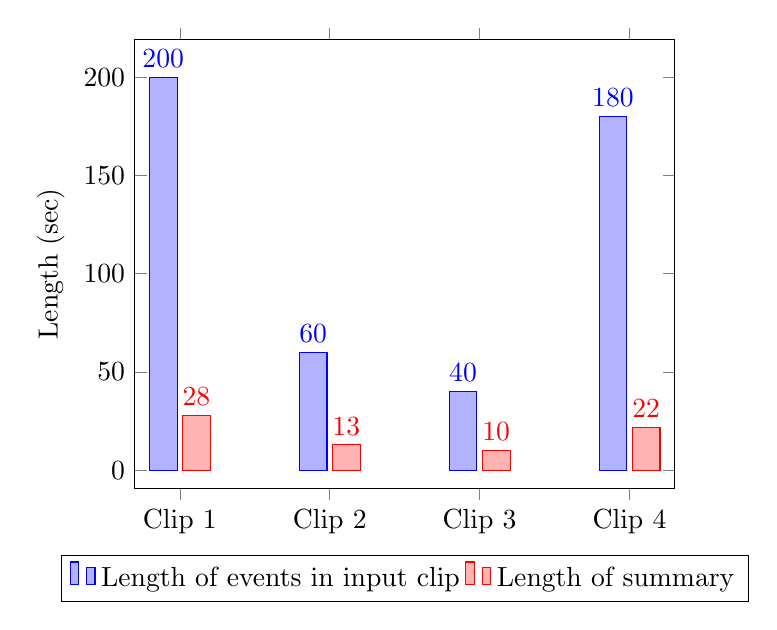
\begin{tikzpicture}
                \begin{axis}[
                    ybar,
                    enlargelimits=0.1,
                    legend style={
                        at={(0.5,-0.15)},
                        anchor=north,legend columns=-1
                    },
                    ylabel={Length (sec)},
                    symbolic x coords={Clip 1, Clip 2, Clip 3, Clip 4},
                    xtick=data,
                    nodes near coords,
                    nodes near coords align={vertical},
                ];
                \addplot coordinates {
                    (Clip 1, 200)
                    (Clip 2, 60)
                    (Clip 3, 40)
                    (Clip 4, 180)
                };
                \addplot coordinates {
                    (Clip 1, 28)
                    (Clip 2, 13)
                    (Clip 3, 10)
                    (Clip 4, 22)
                };
                \legend{Length of events in input clip, Length of summary}

                \end{axis}
            \end{tikzpicture}
        \end{center}


        \item \textbf{Overlap factor}
        A number between 0 and 1 which indicates the amount of overlapping
        (intersection) between the tubes in the summary video. 0 indicates no
        overlap and 1 indicates complete overlap of every clip. \\
        Result: All videos have overlap lower than 0.1
    \end{itemize}

    \subsection{Subjective Evaluation Parameters}

    \begin{itemize}
        \item \textbf{Semantic structure of events}
        Interacting events (that occur in the same time and space) must be
        shown together. \\
        Result: All the interacting events are always shown together
        \item \textbf{Realistic appearance}
        The events must be extracted and be blended into the background
        seamlessly and appear realistic. \\
        Result: Realistic appearance in most cases, with some halo around
        object when at the edges of the frame, or when there is intersection.
    \end{itemize}

    \subsubsection{Performance of Simulated Annealing}
    The simulated annealing optimisation process is not very effective when
    there are a large number of tubes to be re-arranged. The process is
    sensitive to the initial configuration and in some edge cases an optimal
    solution is not obtained. This causes the events in the summary to be
    overlapped. Further improvement in the generation of new configurations and
    an improved cost function will solve the issues faced.

\pagebreak

\section{Summary}

This video summary system which has been developed performs in real-time (30fps)
for the real-time phase and runs reasonably fast in the query phase as well. It
takes about 1 minute for generating a summary video of 10-15 secs.
The outputs are acceptable for the regular summarization (with all events) and
the tag-based summarization, except a few cases where small or fast-moving
objects are not detected. The optimization and blending process can be
improved further to ensure that overlap is further reduced.

    \chapter{Conclusion to CCTVVS}

This project aimed to use a novel method to generate video summaries to reduce
the amount of time spent in analyzing CCTV video footage. Our implementation of
summarization by temporal rearrangement of events improves on other methods of
just detecting frames of motion. The tag-based summary selects only the required
type of event, reducing the summary length further.

A proof-of-concept has been presented, and it can be extended to be used in
commercial CCTV systems with further development.

\section{Limitations of the Project}

While the current system works well for small clips, there are limitations which
prevent it from being used in CCTV system:
    \begin{itemize}
        \item Optimization algorithm doesn’t work very well when there are many
        events
        \item Blending algorithm doesn’t make the summary look perfectly natural
        \item Further performance improvements required for optimization phase,
        to make it run faster
    \end{itemize}

\section{Future Enhancement}

To overcome the limitations of the project, the following will be taken up in
the future:
    \begin{itemize}
        \item Improve performance by parallelising and optimizing the code
        \item Experimenting and improving the optimization algorithm for better
        results with lesser overlap
        \item A simple UI for selecting the input, and setting the parameters
        for the summary is required, with links to go back to the original video
    \end{itemize}

\section{Summary}
This chapter gives an overlook of the entire video summary system and briefly
states the limitation of the project and future enhancements to grow and
overcome the limitations of the same.


% KP
% \cite{reid1959medical}\\
% \cite{sippel2011use}\\
% \cite{bharath2015portable}\\
% \cite{wells2006ultrasound}\\
% \cite{teeter1999user}\\
% \cite{xudong2007user}\\
% \cite{nejatimoharrami2017ui}\\
% \cite{xiaohong2008complex}\\
% \cite{xianhong2012application}\\
% \cite{kozminski2012windows}\\
% \cite{li2015application}\\
% \cite{lei2015design}\\
% \cite{syromiatnikov2014journey}\\
% \cite{liu2015use}\\
% \cite{jambunatha2015design}\\
% \cite{lu2008development}\\
% \cite{moreira2013pattern}\\
% \cite{condren2006automation}\\
% \cite{srivastava2017scrum}\\
% \cite{qureshi2012agile}\\
% \cite{liubchenko2016review}\\
% \cite{ferreira2007agile}

% \cite{mandal2018imaging}
% \cite{albu2015benefits}
% \cite{wells2000current}
% \cite{williams1983brief}
% \cite{rathinam2017review}
% \cite{blahuta2012ultrasound}
% \cite{wu2012combining}
% \cite{loch1999artificial}
% \cite{ogawa1998computer}
% \cite{zheng2018transfer}
\end{comment}

\bibliographystyle{IEEEtran} % We choose the "plain" reference style
\bibliography{refs} % Entries are in the "refs.bib" file
\end{document}